\section{Positive Hadron Identification}

% ------------------------------------------
%     introduction body 
% ------------------------------------------

In this note, the authors describe their methodology used to identify positively charged tracks as one of three common species (pion, kaon, proton), and negatively charged tracks as one of two options (pion, kaon).  Particle identification is the process of combining detector level information, as well as higher level information from the results of reconstruction (charge, momentum, and time of flight) to catagorize each track as a known particle.  These particles can then be corrected and used in physics analyses. \\

First, electrons are identified and any additional (not electrons) tracks in the event are processed.  Second, cuts are applied to remove tracks in poorly understood regions of the detector.  An additional cut is used for our analyses which restricts the vertex of the track to be close to that of the electron.  Such a cut should be removed to study processes with detached vertex positions (arising from the decay of other produced hadrons). Next, the species of particle is chosen based on the likelihood ratio.  Finally, a minimum confidence level for each track is required.  \\

The likelihood methodology described in this note is based on the discussion provided by the BES collaboration \cite{bes_physics}.  

\subsection{Preliminary Cuts}

% ----------------------------------------------
%        cuts used before likelihood 
% ----------------------------------------------

After electron identification, all remaining tracks are subject to two constraints.  First, events which pass close to the torus coils are removed by cutting on the hit positions reported by the region 1 drift chambers, this is shown in figure \ref{fig:fid}.  Such events are often poorly reconstructed or have poorly understood acceptances and are discarded from analyses.  Then, the distance between the electron vertex and the hadron candidate track vertex is computed ($\delta v_{z} = v_{z}^{e} - v_{z}^{+}$).  This distance is constrained to be within the length of the target (5 cm) see figure \ref{fig:dvz}.  As stated above, if the analyst desires to look at events where the hadron is produced as the result of a decaying hadron, this cut should be removed.  

\begin{figure}
  \label{fig:dvz}
  \begin{center}
    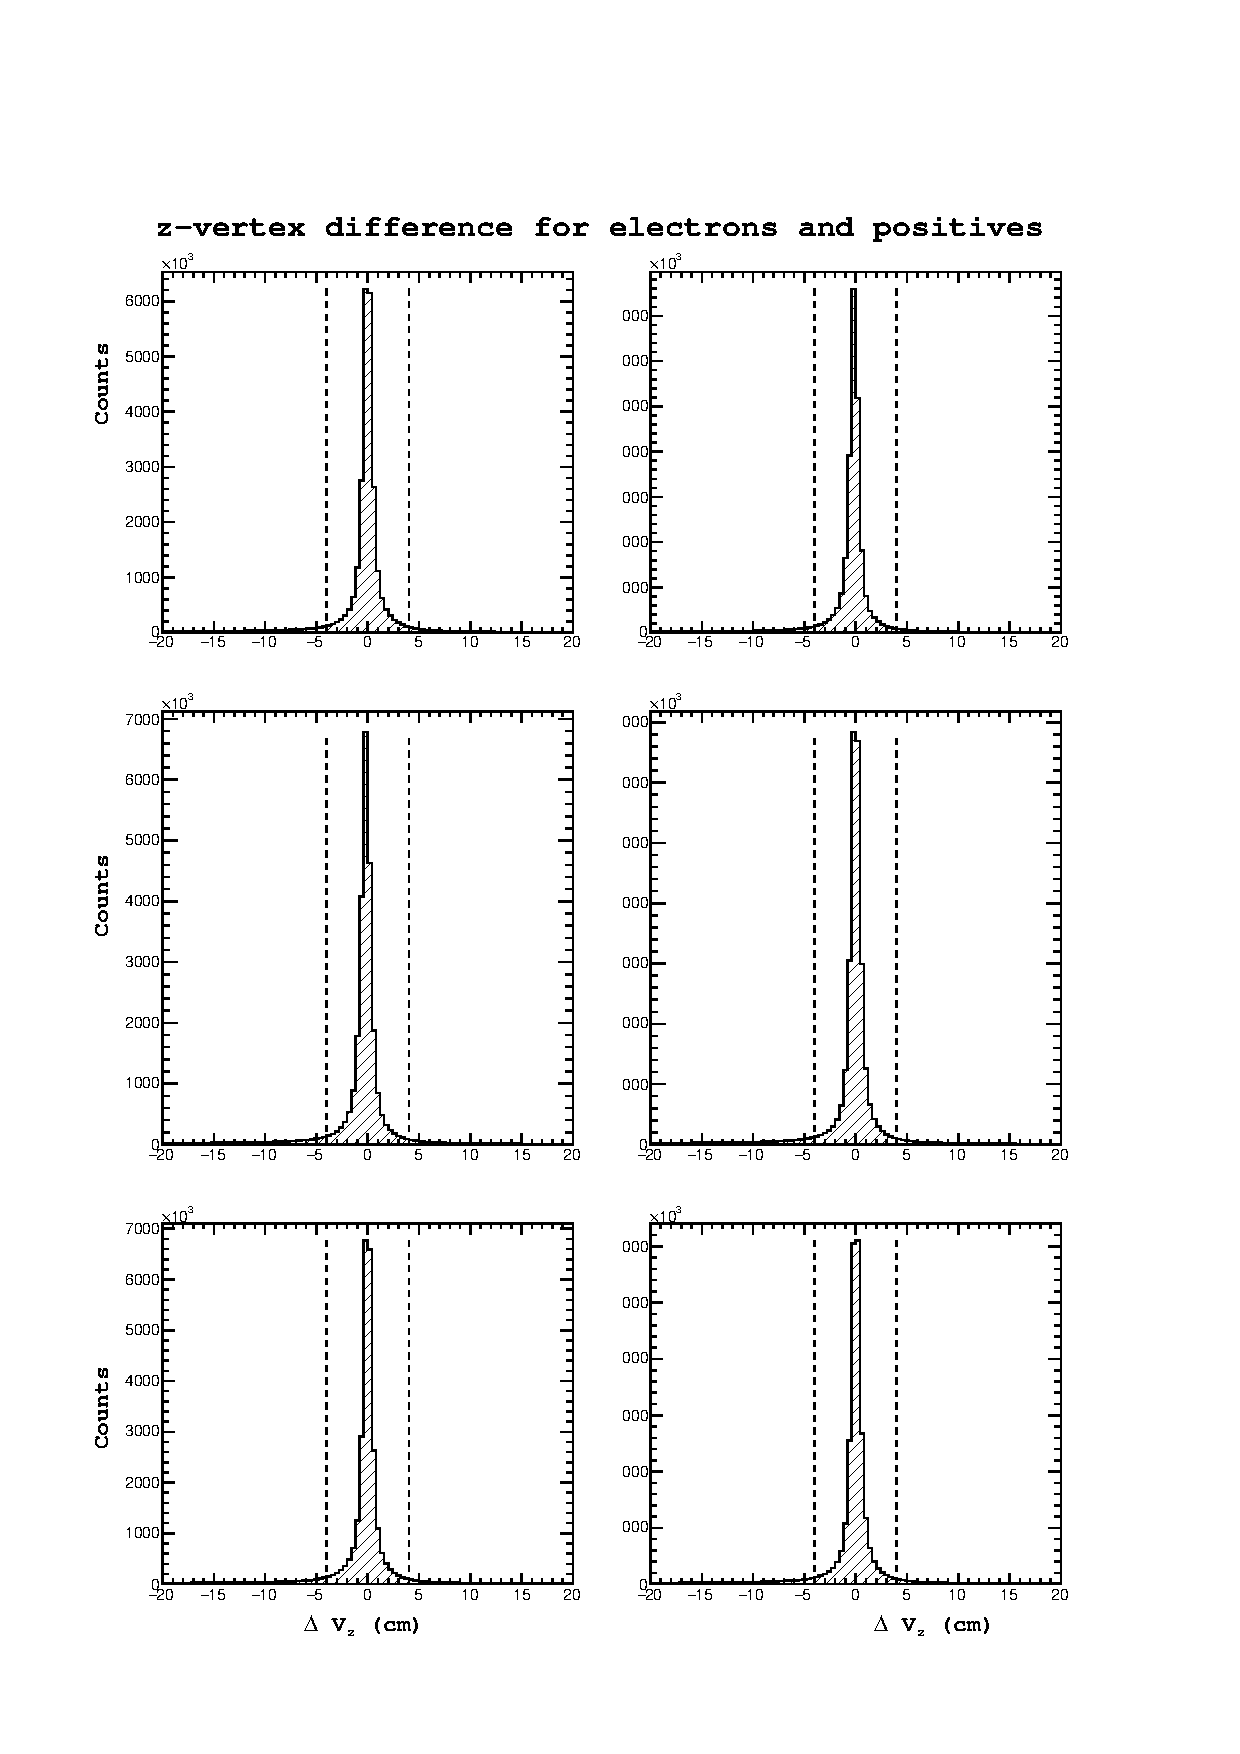
\includegraphics[width=10cm]{image/dvz.pdf}
    \caption{Shown above: The difference between the z-vertex position between detected electrons and positive tracks.}
  \end{center}
\end{figure}

\begin{figure}
  \label{fig:fid}
  \begin{center}
    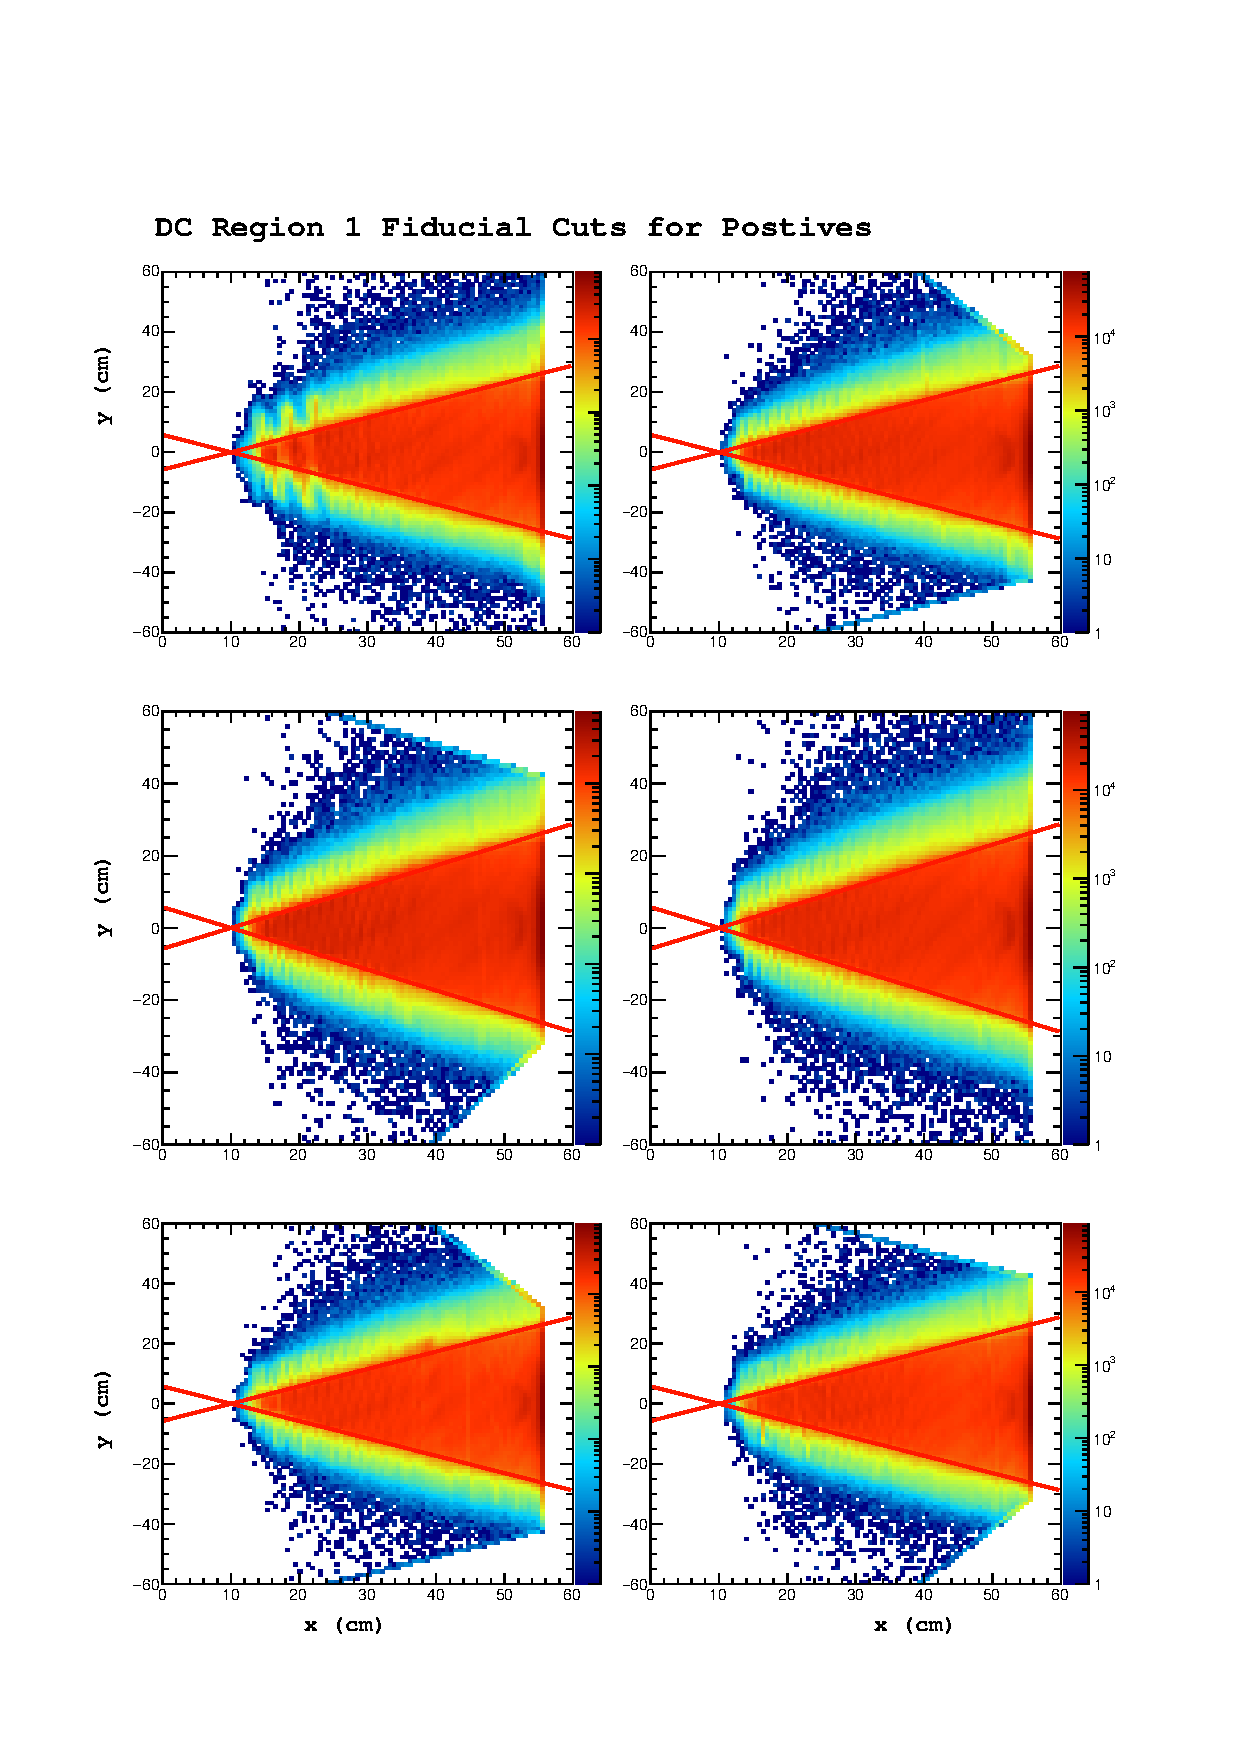
\includegraphics[width=10cm]{image/fid.pdf}
    \caption{Shown above: Positive track hits on the region 1 drift chamber, events falling between the red lines are kept for analysis.}
  \end{center}
\end{figure}

%
% These really don't add anything to the discussion 
%
%\begin{figure}
%  \begin{center}
%    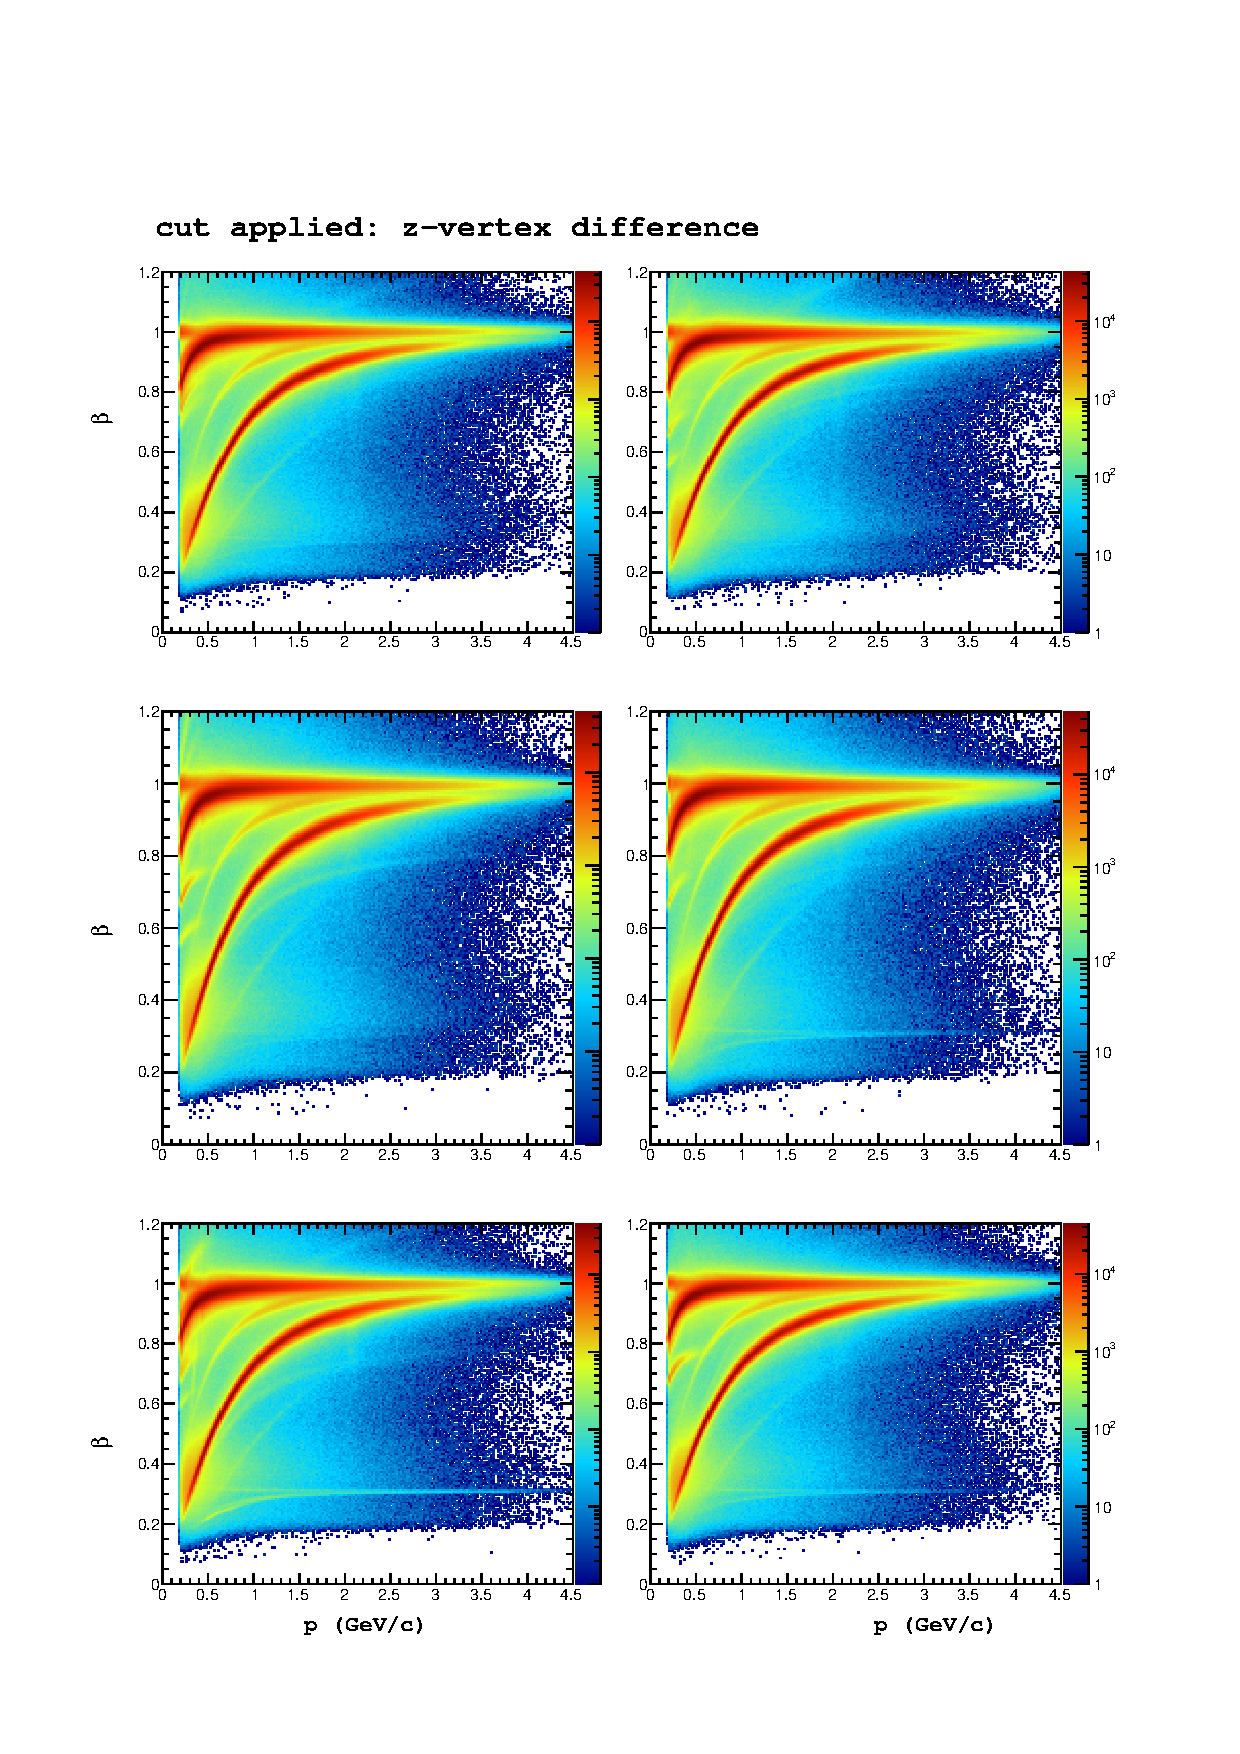
\includegraphics[width=10cm]{image/p_beta_dvz.pdf}
%    \caption{Shown above: }
%  \end{center}
%\end{figure}

%\begin{figure}
%  \begin{center}
%    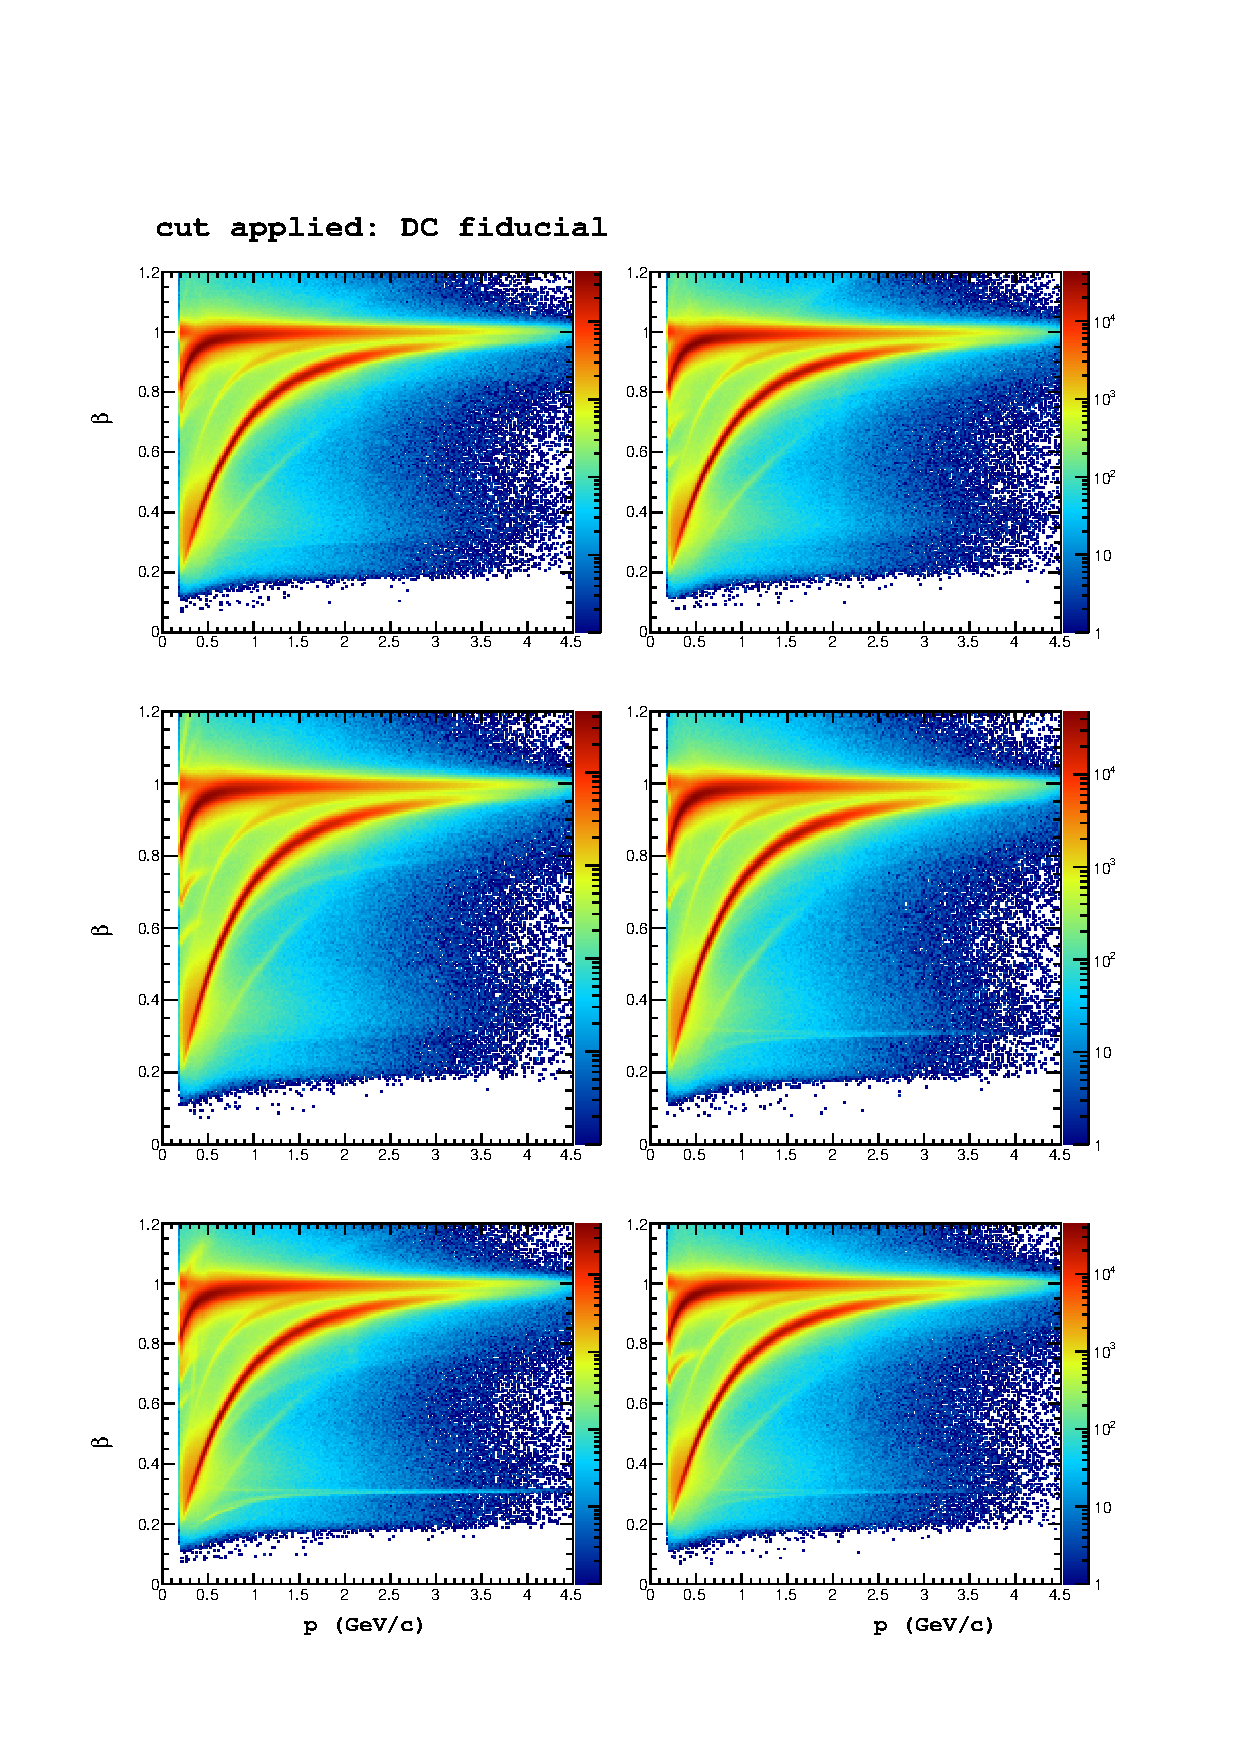
\includegraphics[width=10cm]{image/p_beta_fid.pdf}
%    \caption{Shown above: }
%  \end{center}
%\end{figure}

\subsection{Likelihood Method}
In this section, positive hadrons are used as an example.  The same method is applied to the negative hadrons.  For each particle species considered, a normalized probability density function $P(x;p,h)$ is constructed for each input into the likelihood analysis.  Here, x corresponds to the feature being used to catagorize different particles (in our case, x is the $\beta$ value measured by CLAS time-of-flight), p is the particle momentum, and h is the hadron being hypothesized (eg: in our case the possible values for positive hadrons are pion, kaon, proton).  In general if one uses a set of $N$ variables $x = (x_1, x_2, ..., x_N)$, the likelihood for a hypothesis h is defined below.

\begin{equation}
  \mathcal{L}_h = \prod^{N}_{i=1} P_{i} (x_i; p, h)
\end{equation}

In our case, the only random variable we consider is $\beta$, and the likelihood is just the PDF.  Here, and in many cases where the choice is statistically appropriate, it is possible to use a Gaussian PDF for the variable $x_i$ ($\beta$).

\begin{equation}
  P(\beta;p,h) = \frac{1}{\sqrt{2 \pi} \sigma_\beta(p,h) } exp \left \{ -\frac{1}{2} \bigg( \frac{\beta - \mu_\beta(p,h)}{\sigma_\beta(p,h)} \bigg)^2 \right \}
\end{equation}

The identity is assigned by choosing the particle hypothesis h which maximizes the likelihood ratio.  
 
\begin{equation}
  \frac{\mathcal{L}_h}{\mathcal{L}_{\pi}+\mathcal{L}_{K}+\mathcal{L}_{p}}
\end{equation}

Using this method, every positive track is assigned a particle identification.  However, at times the likelihood value is quite small when compared with the maximum likelihood for that species.  This is the case for positrons which are classified by this method as positive pions, because they are the closest particle for which a hypothesis has been provided.  To avoid these situations, the confidence level $\alpha$ of each track is calculated and a cut is applied on the minimum confidence.  This cut can be easily varied to see how it changes the analysis result.

\begin{equation}
  \alpha = 1 - \int_{\mu-\beta_{obs}}^{\mu+\beta_{obs}} P(\beta;p,h) d\beta
\end{equation}

This quantity represents the probability to observe a value of $\beta$ as far from the mean as $\beta_{obs}$.  Confidence levels of 0 then correspond to tracks which are poorly identified as the class h.  In the case that the PDF is Gaussian, the standard 1, 2, and 3 sigma cuts on $\beta$ vs. $p$ can be understood simply as confidence levels of approximately 0.32 = 1-0.68, 0.05 = 1-0.95, and 0.01 = 1-0.99.

\begin{figure}
  \begin{center}
    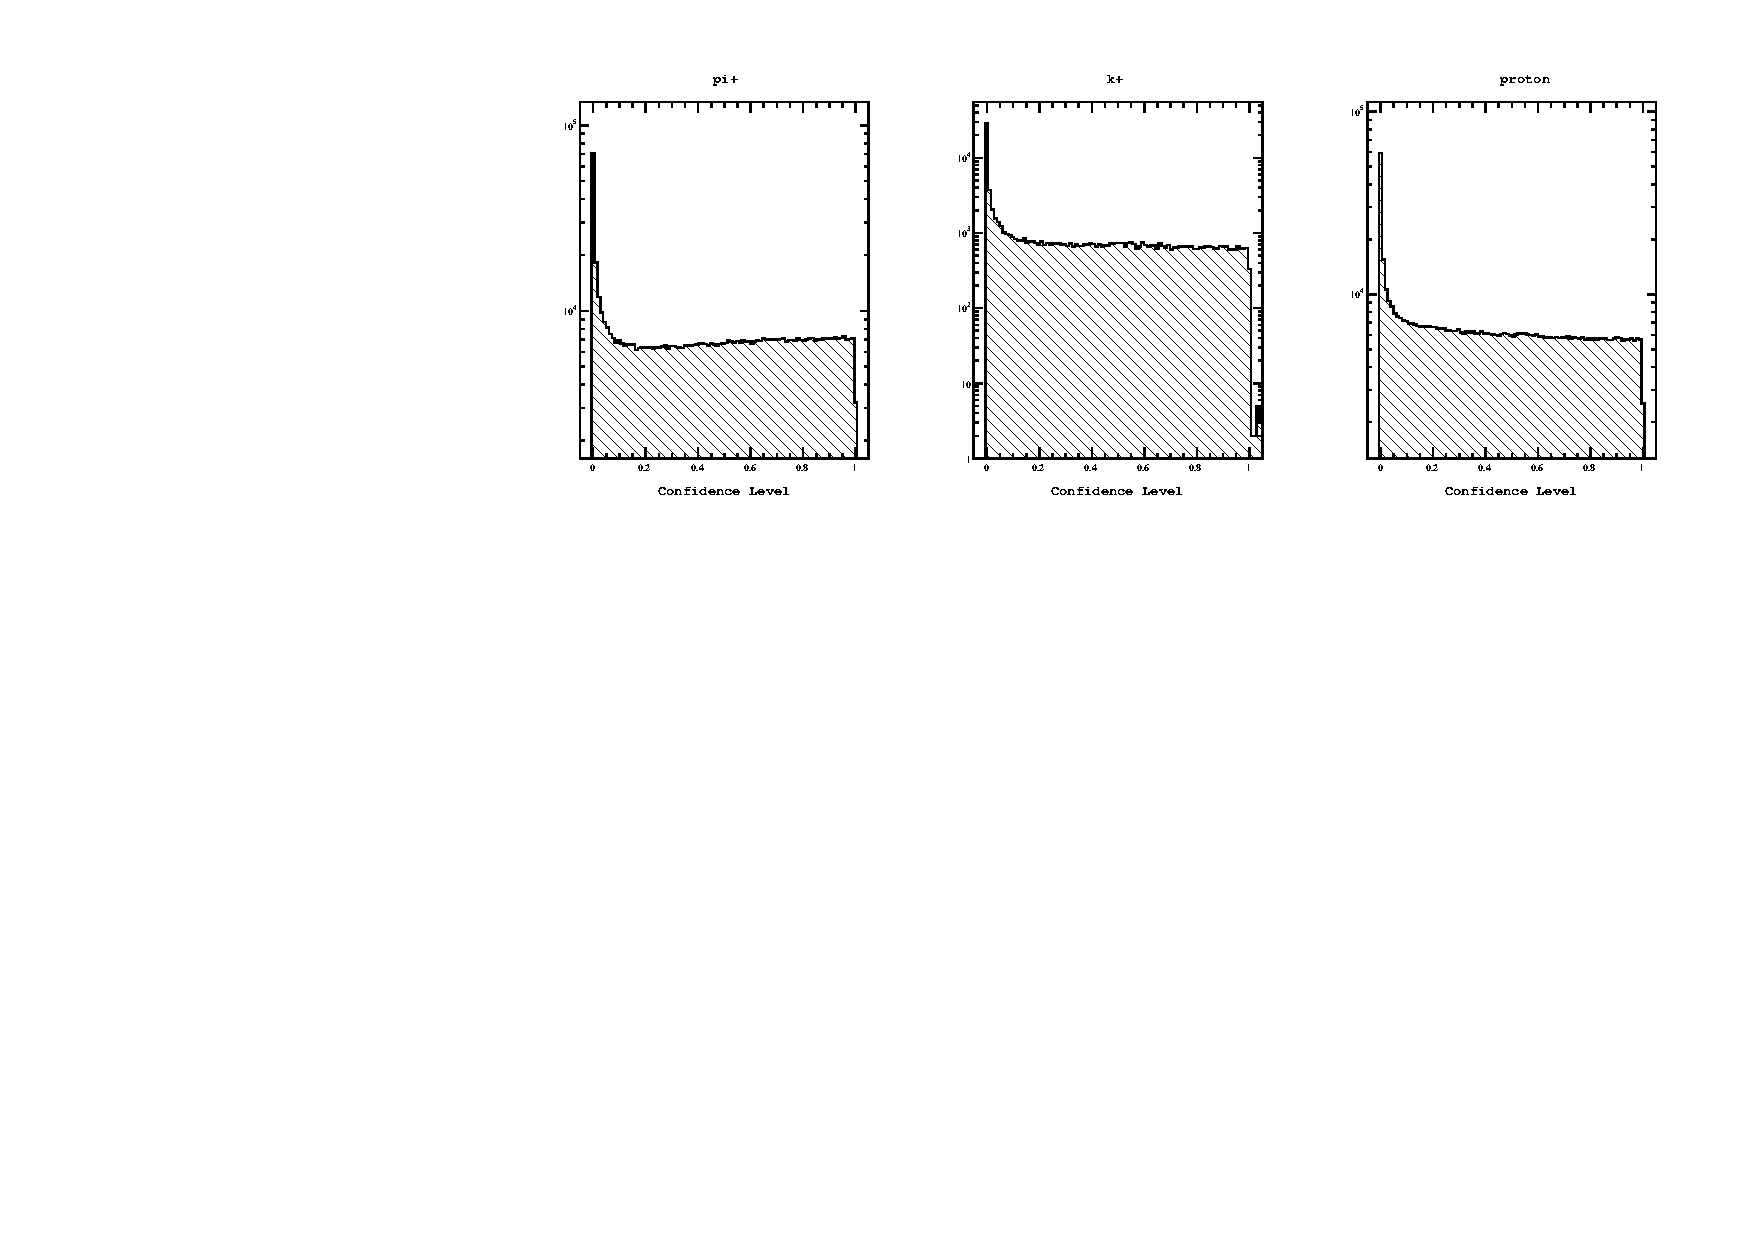
\includegraphics[width=14cm]{image/confidence_level.pdf}
    \caption{ Shown above: The distribution of significance level for all positive tracks after being classified by the likelihood ratio.}
  \end{center}
\end{figure}

\subsection{Determination of Probability Density Functions}

The most important and most difficult part of constructing the likelihood ratio identification is the ascertation of the mean and standard deviation of the probability density function (which depends on momentum) for the different particle hypothesis.  In the case where exceptionally accurate monte carlo (MC) simulations of the detector are available, one can use the truth information and track matching to construct the $\beta$ vs. $p$ 2-dimensional histograms, and fit the $\mu(p)$ and $\sigma(p)$.  In the absence of high quality MC, analysts typically fit directly the spectrum of $\beta$ vs. $p$ and extract the mean and variance.  In this work, the authors chose to create an enhanced sample of candidates for each of the three positive particles in question before doing the fitting.  In this way, we hope to get a better quality fit of the true mean, and resolutions for the different species.  For fitting of pion and proton resolutions, positive tracks are assumed to be pions and the missing mass of the event is calculated.  Then, a cut is placed around the neutron mass.  In doing so, we are selecting mainly two types of exclusive events.  The first is $ep \rightarrow e\pi^+N$, and the second is $ep \rightarrow ep\pi^0$.  In this way most positrons, and positive kaons are removed from the sample prior to fitting.  The mean and variance are fit using a third order polynomial in p (MINUIT $\chi^2$ minimization is used).  The negative tracks $\pi^-$, $K^-$ are fit directly as is normally done.

\begin{figure}
  \begin{center}
    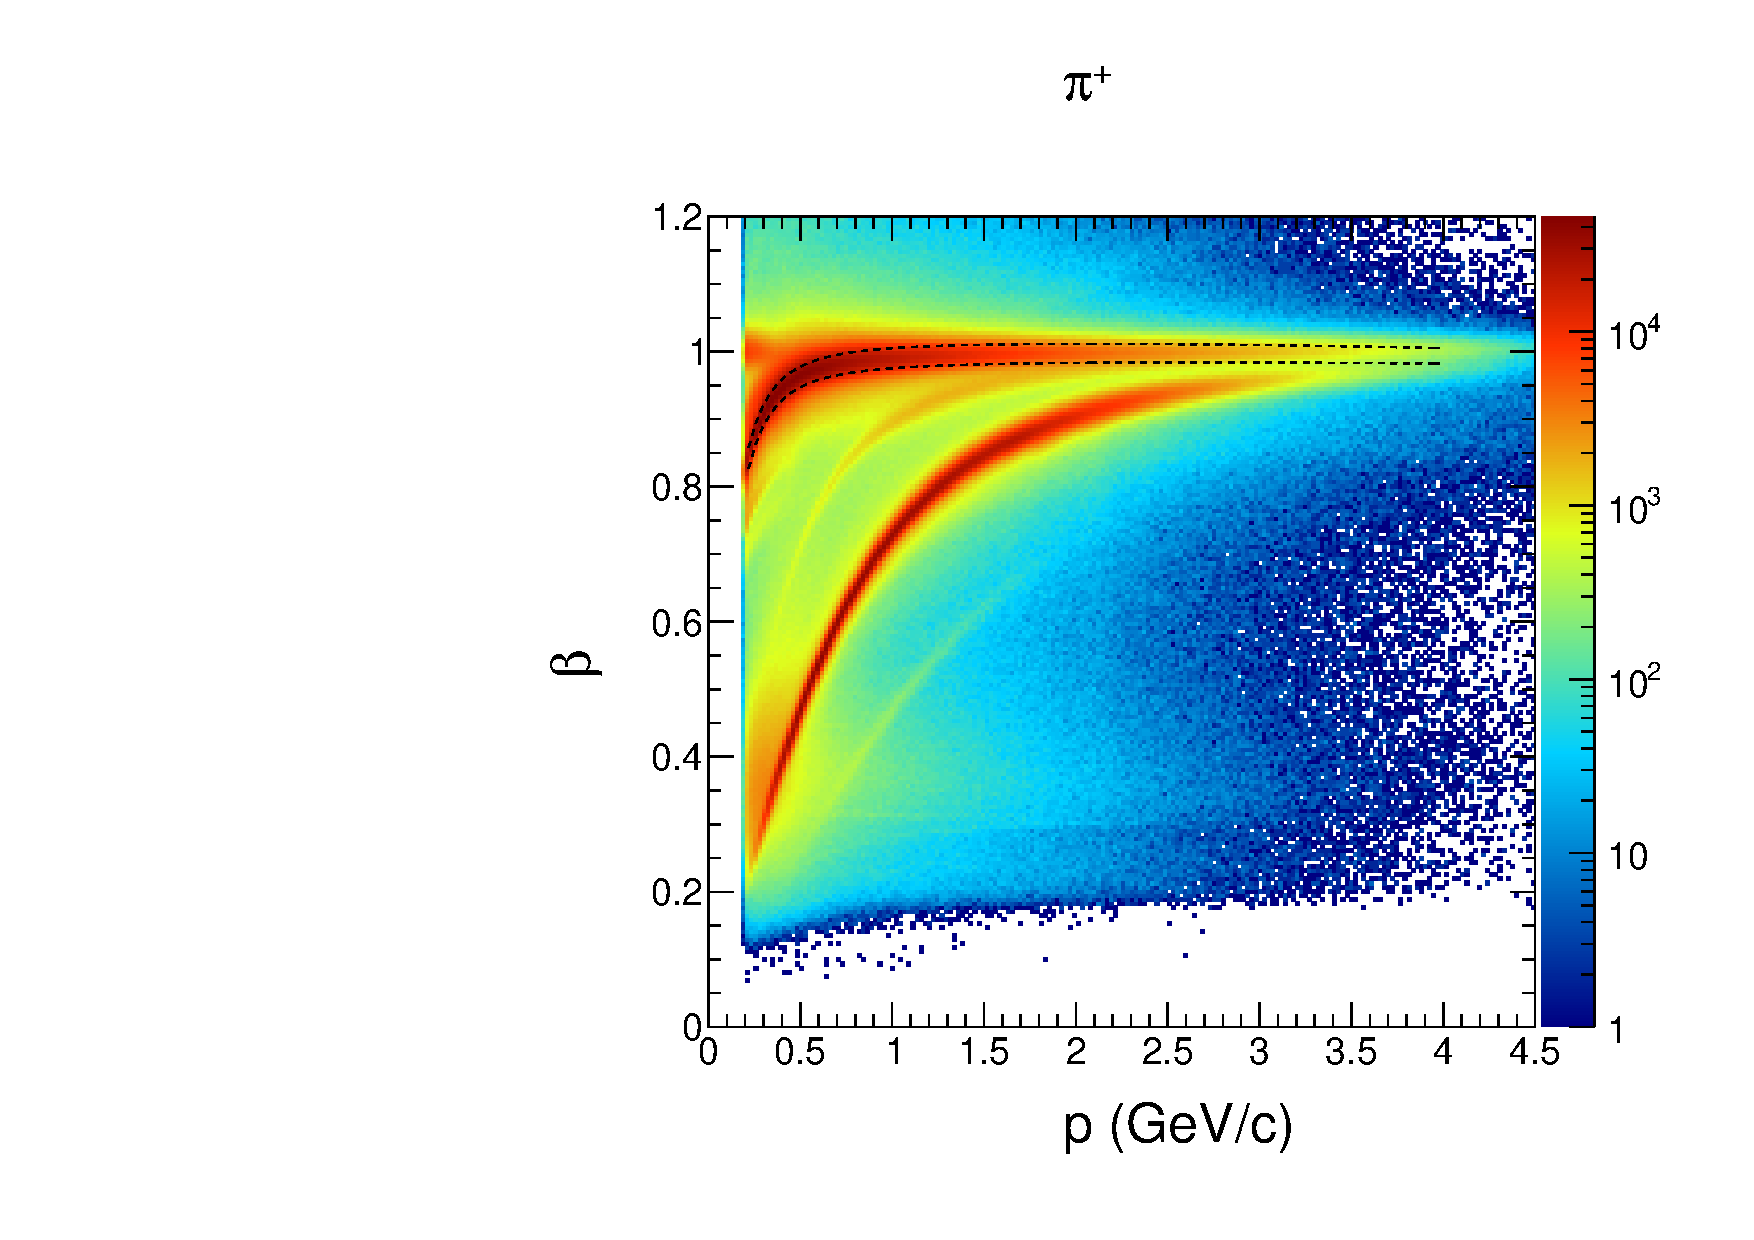
\includegraphics[width=10cm]{image/beautiful_pbeta_pip.pdf}
    \caption{ Shown above: All positive tracks overlaid with our determination of $\mu(p) \pm \sigma(p)$ for $\pi^+$}
  \end{center}
\end{figure}

\begin{figure}
  \begin{center}
    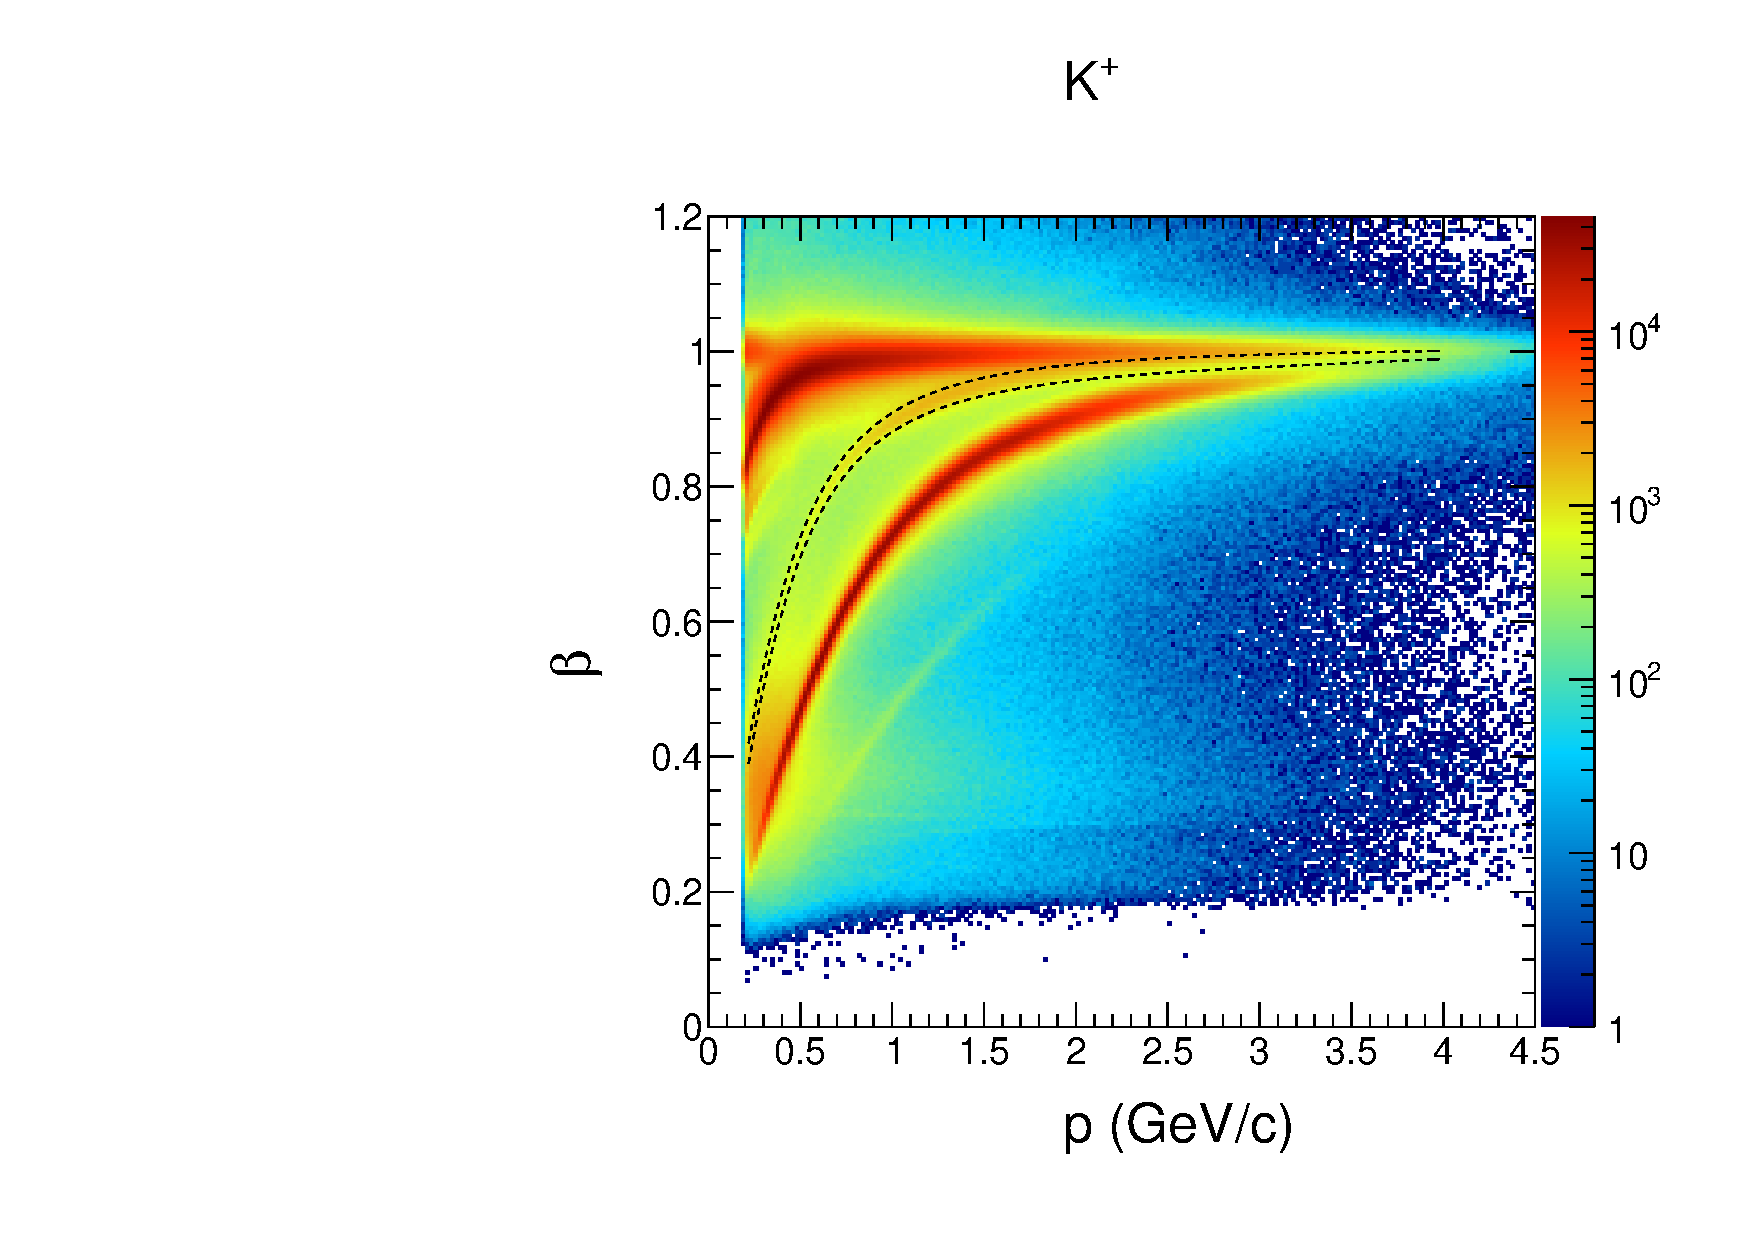
\includegraphics[width=10cm]{image/beautiful_pbeta_kp.pdf}
    \caption{ Shown above: All positive tracks overlaid with our determination of $\mu(p) \pm \sigma(p)$ for $K^+$}
  \end{center}
\end{figure}

\begin{figure}
  \begin{center}
    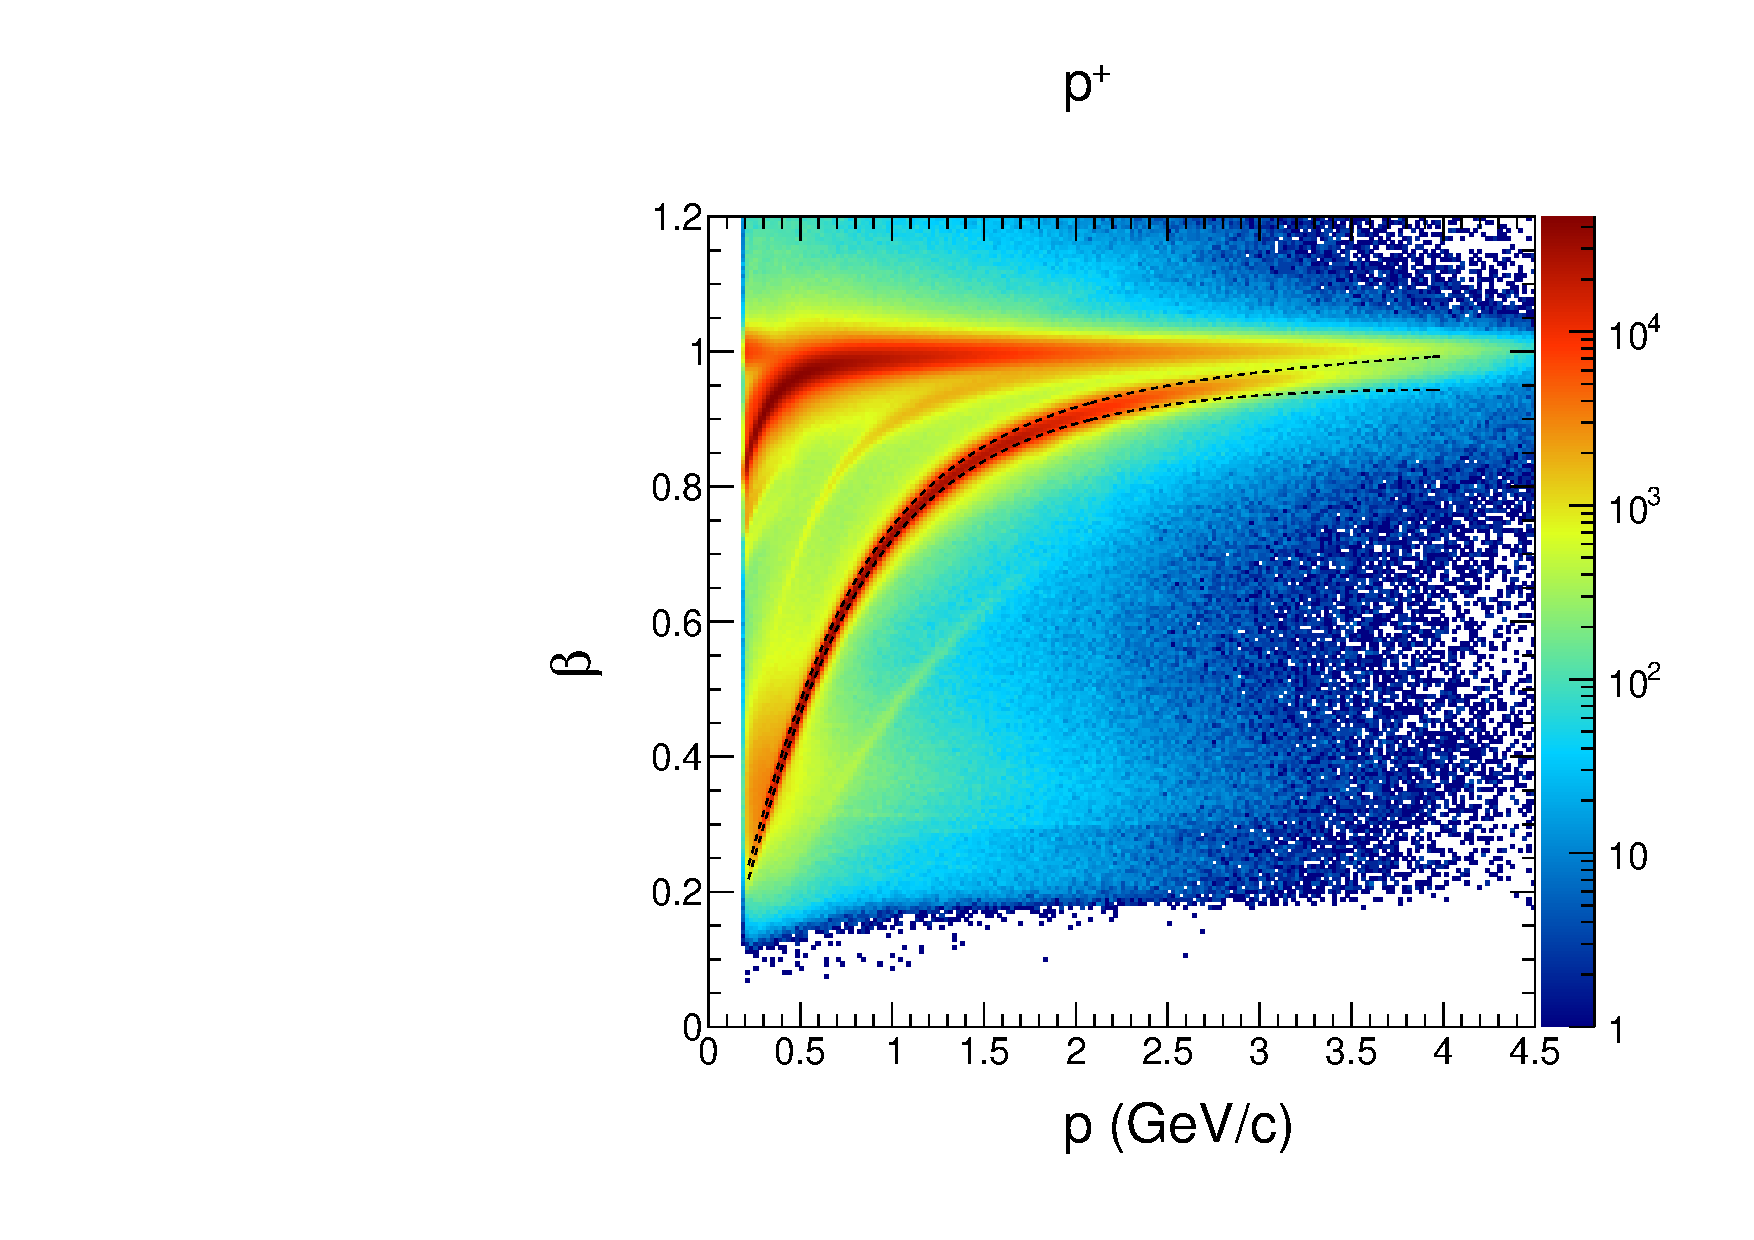
\includegraphics[width=10cm]{image/beautiful_pbeta_prot.pdf}
    \caption{ Shown above: All positive tracks overlaid with our determination of $\mu(p) \pm \sigma(p)$ for $p^+$}
  \end{center}
\end{figure}




